% !Mode:: "TeX:UTF-8:Main"
\documentclass[aspectratio=169]{beamer}

\usepackage{tikzlings}
\usetikzlibrary{calc}
\setbeamertemplate{navigation symbols}{}
\setbeamertemplate{background canvas}{\makebox[\paperwidth]{%
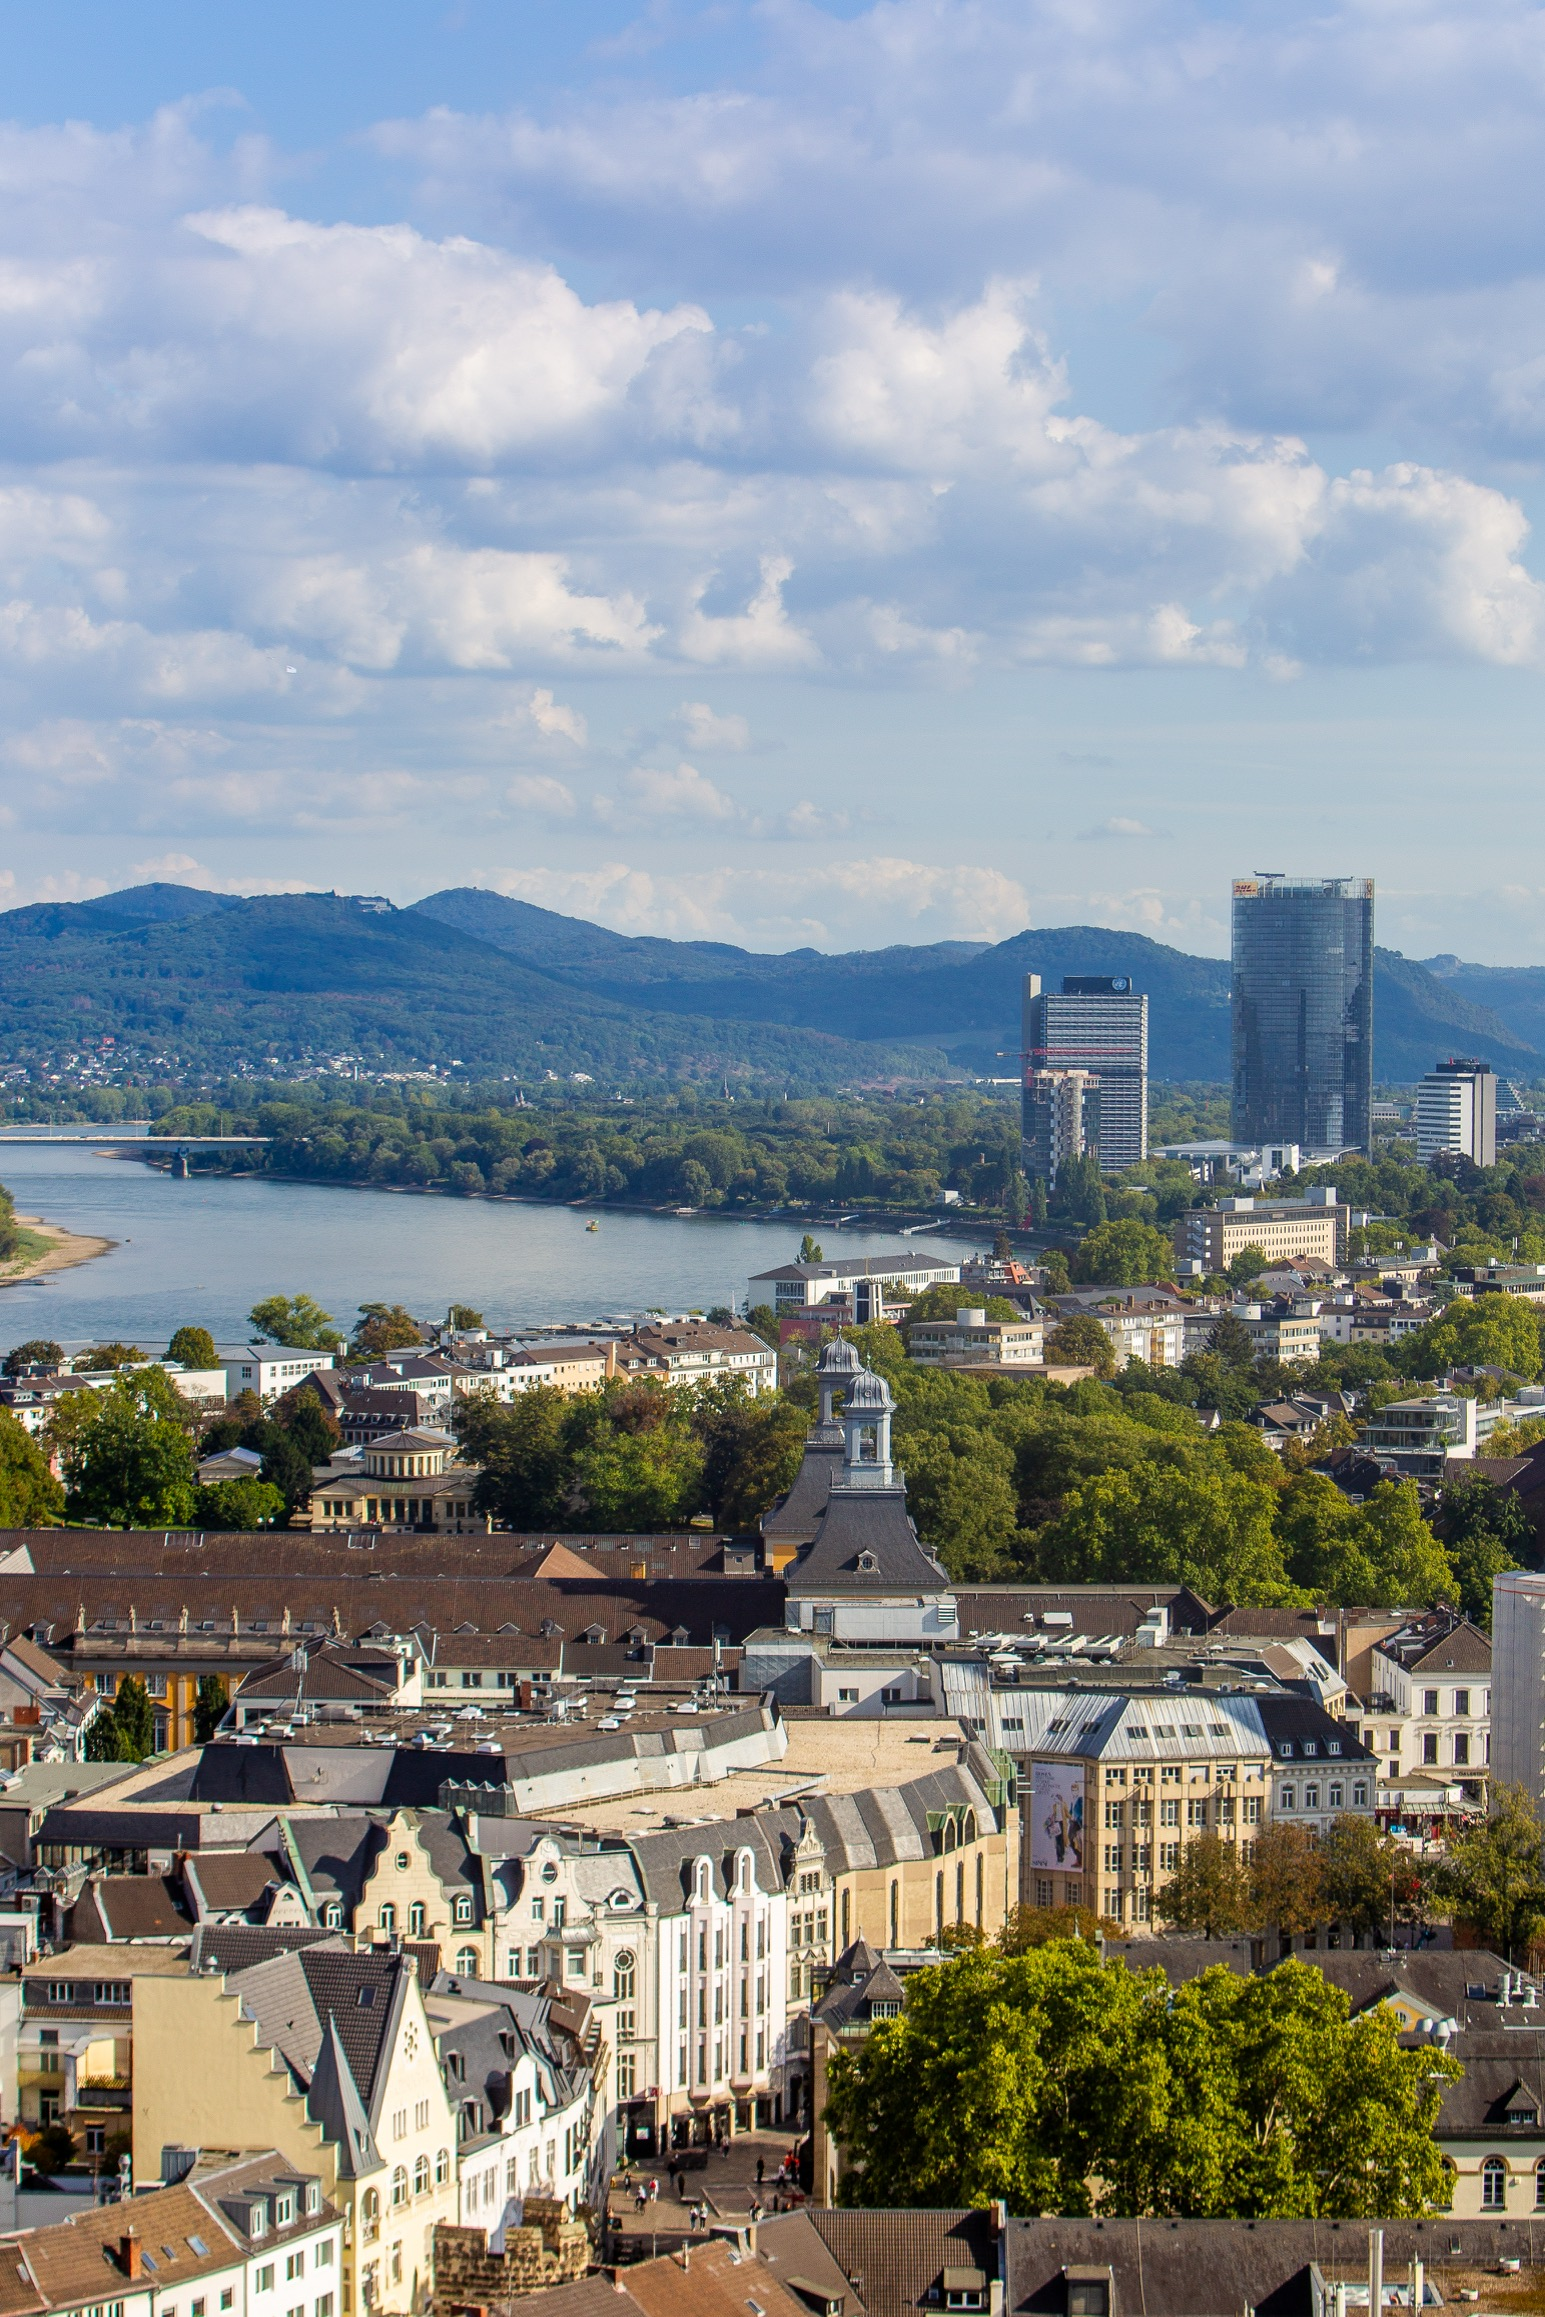
\includegraphics[trim=0cm 12cm 0cm 10cm,height=\paperheight]{bonn}}}

% trick taken from https://topanswers.xyz/tex?q=1989
\tikzset{
    use page relative coordinates/.style={
        shift={(current page.south west)},
        x={(current page.south east)},
        y={(current page.north west)}
    },
}
\usepackage{graphicx,bearwear}
\begin{document}
\begin{frame}
\begin{tikzpicture}[]
\path[use as bounding box](0,0)--(\textwidth,\textheight-14.7pt);
\path[clip]
(0.4\textwidth,\textheight)--(0.65\textwidth,\textheight)--++
(0,-0.38\textheight-10.7pt)--++(-0.15\textwidth,-1.5mm)--++(-0.1\textwidth,2.5mm)--cycle;
  
\begin{scope}[shift={($(0.5\textwidth,0.33\textheight)+(0,\fpeval{\the\value{page}/600*0.2}\textheight)$)}]

\bear[signpost={\begin{tabular}{c}TUG\\ 2023\end{tabular}},
signcolour= brown!50!black,
signback=green!40!black]\bearwear[body deco=
{\node at ([yshift=0mm]beartummy)
  {
\includegraphics[width=0.6cm]{kussmund}};
}]

\end{scope}
\end{tikzpicture}
\pause[600]
\end{frame}
\end{document}
https://m.youtube.com/watch?v=O7Iu5Vyo1us 0.0--030 
